\documentclass[aspectratio=169]{../latex_main/tntbeamer}  % you can pass all options of the beamer class, e.g., 'handout' or 'aspectratio=43'
\usepackage{dsfont}
\usepackage{bm}
\usepackage[english]{babel}
\usepackage[T1]{fontenc}
%\usepackage[utf8]{inputenc}
\usepackage{graphicx}
\graphicspath{ {./figures/} }
\usepackage{algorithm}
\usepackage[ruled,vlined,algo2e,linesnumbered]{algorithm2e}
\usepackage{hyperref}
\usepackage{booktabs}
\usepackage{mathtools}

\usepackage{amsmath,amssymb}

\DeclareMathOperator*{\argmax}{arg\,max}
\DeclareMathOperator*{\argmin}{arg\,min}

\usepackage{pgfplots}
\pgfplotsset{compat=1.16}
\usepackage{tikz}
\usetikzlibrary{trees} 
\usetikzlibrary{shapes.geometric}
\usetikzlibrary{positioning,shapes,shadows,arrows,calc,mindmap}
\usetikzlibrary{positioning,fadings,through}
\usetikzlibrary{decorations.pathreplacing}
\usetikzlibrary{intersections}
\pgfdeclarelayer{background}
\pgfdeclarelayer{foreground}
\pgfsetlayers{background,main,foreground}
\tikzstyle{activity}=[rectangle, draw=black, rounded corners, text centered, text width=8em]
\tikzstyle{data}=[rectangle, draw=black, text centered, text width=8em]
\tikzstyle{myarrow}=[->, thick, draw=black]

% Define the layers to draw the diagram
\pgfdeclarelayer{background}
\pgfdeclarelayer{foreground}
\pgfsetlayers{background,main,foreground}

% Requires XeLaTeX or LuaLaTeX
\usepackage{unicode-math}

\usepackage{fontspec}
%\setsansfont{Arial}
\setsansfont{RotisSansSerifStd}[ 
Path=../latex_main/fonts/,
Extension = .otf,
UprightFont = *-Regular,  % or *-Light
BoldFont = *-ExtraBold,  % or *-Bold
ItalicFont = *-Italic
]
\setmonofont{Cascadia Mono}[
Scale=0.8
]

% scale factor adapted; mathrm font added (Benjamin Spitschan @TNT, 2021-06-01)
%\setmathfont[Scale=1.05]{Libertinus Math}
%\setmathrm[Scale=1.05]{Libertinus Math}

% other available math fonts are (not exhaustive)
% Latin Modern Math
% XITS Math
% Libertinus Math
% Asana Math
% Fira Math
% TeX Gyre Pagella Math
% TeX Gyre Bonum Math
% TeX Gyre Schola Math
% TeX Gyre Termes Math

% Literature References
\newcommand{\lit}[2]{\href{#2}{\footnotesize\color{black!60}[#1]}}

%%% Beamer Customization
%----------------------------------------------------------------------
% (Don't) Show sections in frame header. Options: 'sections', 'sections light', empty
\setbeamertemplate{headline}{empty}

% Add header logo for normal frames
\setheaderimage{
	% 
\includegraphics[height=\logoheight]{figures/TNT_darkv4.pdf}
	
\includegraphics[height=\logoheight]{../latex_main/figures/luh_logo_rgb_0_80_155.pdf}
	% 
\includegraphics[height=\logoheight]{figures/logo_tntluh.pdf}
}

% Header logo for title page
\settitleheaderimage{
	% 
\includegraphics[height=\logoheight]{figures/TNT_darkv4.pdf}
	
\includegraphics[height=\logoheight]{../latex_main/figures/luh_logo_rgb_0_80_155.pdf}
	% 
\includegraphics[height=\logoheight]{figures/logo_tntluh.pdf}
}

% Title page: tntdefault 
\setbeamertemplate{title page}[tntdefault]  % or luhstyle
% Add optional title image here
%\addtitlepageimagedefault{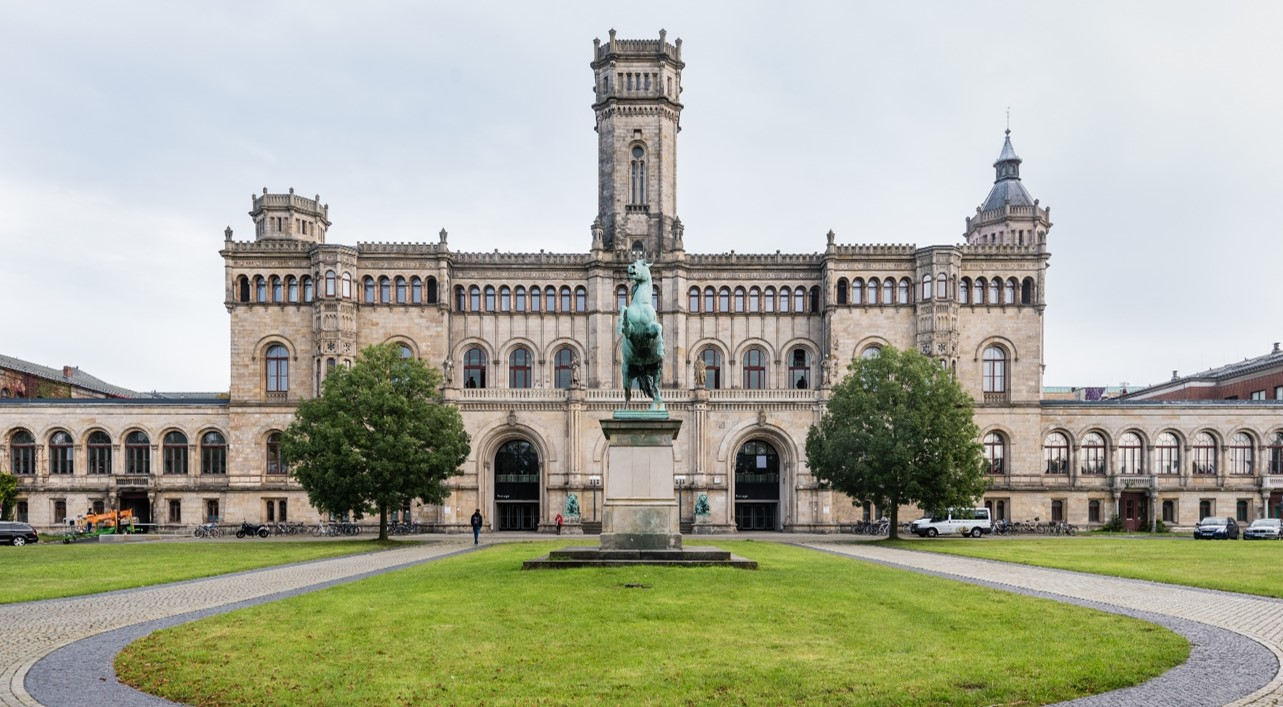
\includegraphics[width=0.65\textwidth]{figures/luh_default_presentation_title_image.jpg}}

% Title page: luhstyle
% \setbeamertemplate{title page}[luhstyle]
% % Add optional title image here
% \addtitlepageimage{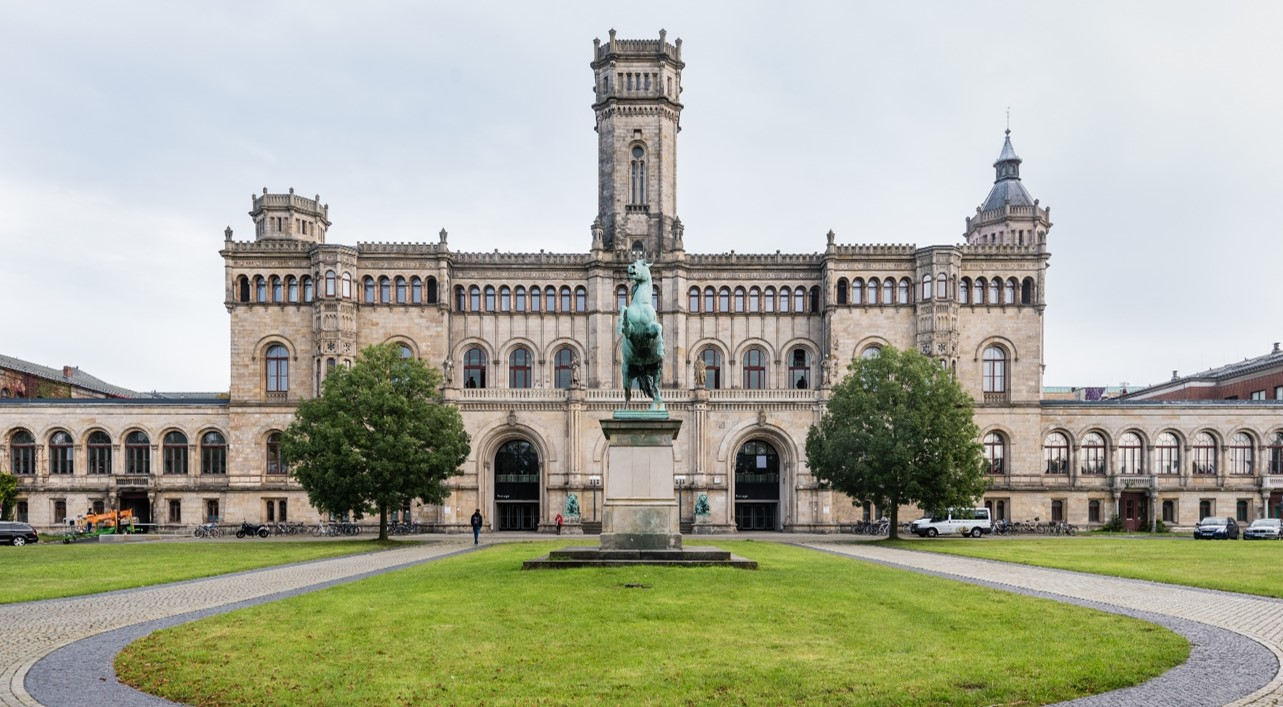
\includegraphics[width=0.75\textwidth]{figures/luh_default_presentation_title_image.jpg}}

\author[Lindauer \& Anand]{Marius Lindauer and Avishek Anand\\[1em]
	
\includegraphics[height=\logoheight]{../latex_main/figures/luh_logo_rgb_0_80_155.pdf}\qquad

\includegraphics[height=\logoheight]{../latex_main/figures/TNT_darkv4}\qquad

\includegraphics[height=\logoheight]{../latex_main/figures/L3S.jpg}	}
\date{Winter Term 2021
}


%%% Custom Packages
%----------------------------------------------------------------------
% Create dummy content
\usepackage{blindtext}

% Adds a frame with the current page layout. Just call \layout inside of a frame.
\usepackage{layout}


\title[Introduction]{iML: Feature Effects}
\subtitle{ALE}

%\institute{}


\begin{document}
	
	\maketitle

	%-----------------------------------------------------------------------------------------------------------------------------

\begin{frame}[c]{Motivation}

\begin{center}
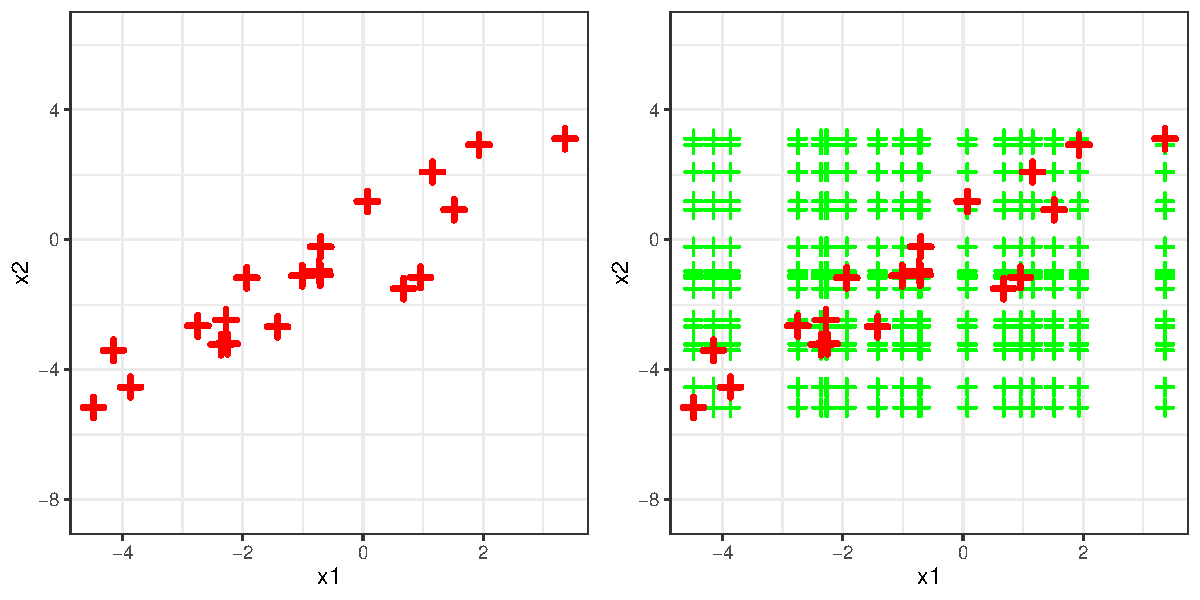
\includegraphics[width=0.5\textwidth]{figure/pd_grid}
\end{center}

\textbf{Recall:} In case of strongly correlated features $x_1$ and $x_2$, partial dependence (PD) plots \textbf{average predictions} of artificial data instances that are unlikely in reality (green).
This can lead to biased estimates.

\textbf{Question:} Can we avoid the extrapolation issue by averaging only over points in the neighborhood of a specific point $x_1$? 

\end{frame}
%----------------------------------------------------------------

\begin{frame}[c]{Motivation}

\textbf{Question:} Can we avoid the extrapolation issue by averaging only over points in the neighborhood of a specific point $x_1$? 
\medskip
\pause

\textbf{Answer:} Yes, we could. Marginal plots (M plots) do this by averaging (i.e., marginalizing) over the conditional distribution $P(x_2|x_1)$.

\medskip
\pause

\textbf{But:} M plots introduce the omitted-variable bias (OVB) issue,\\
\begin{itemize}
    \item an M plot always includes the marginal effect of other dependent features.\\
    \item[$\leadsto$] M plots are useless to assess the main effect of a feature in case of dependent features. 
\end{itemize}

\end{frame}

\begin{frame}{Motivation: PD vs. M plot}

\begin{center}
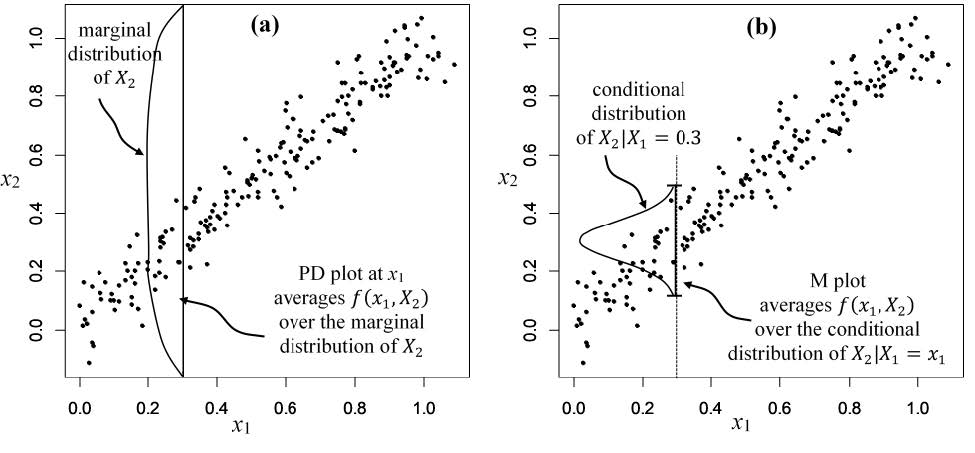
\includegraphics[width=0.5\textwidth]{figure/PD_M.jpg}\\
\tiny{Source: \lit{Apley and Zhu. 2016}{https://arxiv.org/pdf/1612.08468.pdf}}
\end{center}

\begin{enumerate}
\item[a)] PD plot $\hat{f}_{1, PD}(x_1) = \hat{\mathbb{E}}_{x_2} \left( \hat{f}(x_1, x_2) \right) = \frac{1}{n} \sum_{i=1}^n \hat{f}(x_1, x_2^{(i)})$
\item[b)] M plot $\hat{f}_{1, M}(x_1) = \hat{\mathbb{E}}_{x_2|x_1} \left( \hat{f}(x_1, x_2) \middle| x_1\right) = \frac{1}{|N(x_1)|} \sum\limits_{i \in N(x_1)} \hat{f}(x_1, x_2^{(i)})$, where $N(x_1) = \{i: x_1^{(i)} \in [x_1 - \epsilon, x_1 + \epsilon]\}$ is an index set referring to observations in an appropriate neighborhood of feature value $x_1$.
\end{enumerate}

\end{frame}


\begin{frame}{Motivation: PD vs. M plot}

\begin{center}
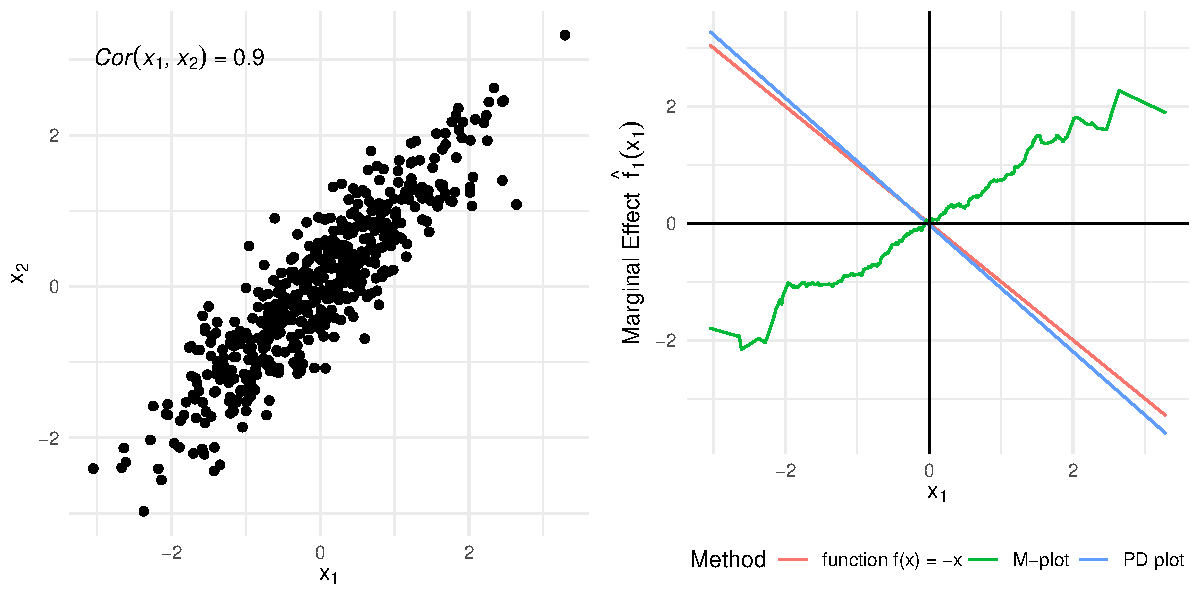
\includegraphics[width=0.45\textwidth]{figure/pd_vs_mplot} %TODO: Font size of tiks and legend
\end{center}

\textbf{Illustration:}
We fitted a linear model on a simulated dataset with 500 i.i.d. observations, features $x_1, x_2 \sim N(0,1)$ with $Cor(x_1, x_2) = 0.9$ and $$y = -x_1 + 2 \cdot x_2 + \epsilon, \; \epsilon \sim N(0,1).$$

\textbf{Results:} The M plot of $x_1$ is a mixture of the marginal effect of $x_1$ and the marginal effect of all other dependent features (here: $x_2$).
\end{frame}

\begin{frame}{Accumulated Local Effects}

Accumulated Local Effect (ALE) plots were developed to overcome the extrapolation issue of PD plots and the OVB issue of M plots when features are dependent \lit{Apley and Zhu. 2016}{https://arxiv.org/pdf/1612.08468.pdf}.

\pause
\medskip
ALE plots are based on:
\begin{enumerate}
\item estimating the local effect $\frac{\partial \hat{f}(x_S, x_C)}{\partial x_S}$ of $x_S$ at $(x_S = z_S, x_C)$,
\pause
\item averaging the local effects across all values of $x_C$, i.e., over the conditional distribution $P(x_C|x_S)$ similar to M plots.\\
$\Rightarrow$ Avoids the extraploation issue.
\pause
\item accumulating/integrating the averaged local effects over all values of $z_S$ up to a specific value $x$ $\Rightarrow$ Avoids the OVB issue.
\end{enumerate}

\end{frame}

%------------------------------------------------------------------

\begin{frame}{Accumulated Local Effects}

\begin{itemize}
    \item Let $z_0$ denote the minimum of observed values of feature $x_S$, i.e., $z_0 = min(x_S)$.
    \item All complementary features are denoted by $x_C$.
    \item The uncentered first order ALE $\tilde{f}_{S, ALE}(x)$ at point $x$ is defined as:
\end{itemize}

$$
\begin{aligned}
\tilde{f}_{S, ALE}(x) &= \int_{z_{0}}^{x} \mathbb{E}_{x_C \vert x_S} \left(\frac{\partial \hat{f}(x_S, x_C)}{\partial x_S} \bigg \vert x_S = z_S \right) dz_S. \\
&= \int_{z_{0}}^{x} \int_{-\infty}^{\infty}  \frac{\partial \hat{f}(z_S, x_C)}{\partial z_S} d P(x_C | z_S) \, dz_S.
\end{aligned}
$$

\end{frame}

%%%%%%%%%%%%%%%%%%%%%%%%%%%%%%%%%%
\begin{frame}{Derivative and Subsequent Integral}
\alert{Idea:} To remove unwanted effects of other features, we take the partial derivative of the prediction function with respect to a feature and integrate it with respect to the same feature. \\
\smallskip\pause
Example:
\begin{itemize}
\item Consider an additive prediction function: $\hat{f}(x_1, x_2) = 2x_1 + 2x_2 - 4x_1 x_2$
\smallskip\pause
\item Partial derivative of $\hat{f}$ with respect to $x_1$: $\frac{\partial \hat{f}(x_1, x_2)}{\partial x_1} = 2 - 4x_2$
\smallskip\pause
\item Integral of the partial derivative:  $\int_{z_0}^{x} \frac{\partial \hat{f}(x_1, x_2)}{\partial x_1} dx_1 = \left[2x_1 - 4x_1 x_2\right]_{z_0}^{x}$
\smallskip\pause
\item[$\leadsto$] We removed the main effect of $x_2$ which was our goal.
\end{itemize}
\end{frame}

%%%%%%%%%%%%%%%%%%%%%%%%%%%%%%%%%%%%

\begin{frame}{First Order ALE}

\vspace{-2em}
\begin{itemize}
    \item Let $z_0$ denote the minimum of observed values of feature $x_S$, i.e., $z_0 = min(x_S)$.
    \item All complementary features are denoted by $x_C$.
    \item The uncentered first order ALE $\tilde{f}_{S, ALE}(x)$ at point $x$ is defined as:
\end{itemize}
  
$$
\begin{aligned}
\tilde{f}_{S, ALE}(x) &= \int_{z_{0}}^{x} \mathbb{E}_{x_C \vert x_S} \left[\frac{\partial \hat{f}(x_S, x_C)}{\partial x_S} \bigg \vert x_S = z_S \right] dz_S \\
&= \int_{z_{0}}^{x} \left[ \int_{-\infty}^{\infty}  \frac{\partial \hat{f}(z_S, x_C)}{\partial z_S} d P(x_C | z_S) \,   \right] dz_S
\end{aligned}
$$

\pause

A constant, i.e., the average of the uncentered ALE curve is substracted such that the centered ALE curve $\hat{f}_{S, ALE}(x)$ has a mean of zero with respect to the marginal distribution of $x_S$:

$$
\begin{aligned}
f_{S, ALE}(x) = \tilde{f}_{S, ALE}(x) - \underbrace{\int_{-\infty}^{\infty}\tilde{f}_{S, ALE}(x_S) \, d P(x_S)}_{:= const}
\end{aligned}
$$

\end{frame}

%%%%%%%%%%%%%%%%%%%%%%%%%%%%%%%%%%%%%

\begin{frame}{PD vs. ALE}
    \textbf{PD:}
    $
    \begin{aligned}
      \hspace{2cm} \mathbb{E}_{x_C} \left( \hat{f}(x_S, x_C) \right) = \int_{-\infty}^{\infty} \hat{f}(x_S, x_C) \, d P(x_C)
    \end{aligned}
    $ \\[2em]
    \textbf{ALE:}
    $
    \begin{aligned}
      \int_{z_{0}}^{x} \mathbb{E}_{x_C \vert x_S} \left[\textcolor{purple}{\frac{\partial \hat{f}(x_S, x_C)}{\partial x_S}} \textcolor{blue}{\bigg \vert x_S = z_S} \right] dz_S\\
        = \int_{z_{0}}^{x} \left[ \int_{-\infty}^{\infty}  \textcolor{purple}{\frac{\partial \hat{f}(x_S, x_C)}{\partial x_S}} d \textcolor{blue}{P(x_C | z_S) } \,   \right] dz_S
  \end{aligned}
    $
    \begin{itemize}
    \item \alert{Difference 1}: PD averages predictions over the marginal distribution while ALE averages the \textcolor{purple}{change} of predictions (defined as the gradient) over the \textcolor{blue}{conditional} distribution.
    \end{itemize}
\end{frame}

%%%%%%%%%%%%%%%%%%%%%%%%%%%%%%%%%%%%%

\begin{frame}{PD vs. ALE}
    \textbf{PD:}
    $
    \begin{aligned}
      \hspace{2cm} \mathbb{E}_{x_C} \left( \hat{f}(x_S, x_C) \right) = \int_{-\infty}^{\infty} \hat{f}(x_S, x_C) \, d P(x_C)
    \end{aligned}
    $ \\[2em]
    \textbf{ALE:}
    $
    \begin{aligned}
    \textcolor{blue}{\int_{z_{0}}^{x}} \mathbb{E}_{x_C \vert x_S} \left[\frac{\partial \hat{f}(x_S, x_C)}{\partial x_S} \bigg \vert x_S = z_S \right] \textcolor{blue}{dz_S}\\
  = \textcolor{blue}{\int_{z_{0}}^{x}} \left[ \int_{-\infty}^{\infty}\frac{\partial \hat{f}(x_S, x_C)}{\partial x_S} d P(x_C | z_S)  \,   \right]
  \end{aligned}
    $
    \begin{itemize}

    \item \alert{Difference 2}: ALE has an additional \textcolor{blue}{integral over $z_S$}. Instead of directly averaging the predictions, the ALE method calculates the prediction differences conditional on features S and integrates the derivative over features $S$ to estimate the effect. The derivative (or interval difference) isolates the effect of the feature of interest and blocks the effect of correlated features.
    \end{itemize}
\end{frame}

%%%%%%%%%%%%%%%%%%%%%%%%%%%%%%%%%

\begin{frame}{ALE Estimation}

\begin{itemize}
  \item Not all models come with a gradient, e.g. random forests.
  \item In order to estimate the first order ALE we have to approximate the partial derivative of the prediction function. We do so by computing finite differences of predictions within a set of $K$ intervals for the value range of observed feature values $x_S$:
  $$
  \begin{aligned}
  x \in [min(x_S), max(x_S)] \iff &x \in [z_{0, S}, z_{1, S}] \\
  \lor &x \in \; ]z_{1, S}, z_{2, S}] \\
  &\dots \\
  \lor &x \in \; ]z_{K-1, S}, z_{K, S}]
  \end{aligned}
  $$
  \pause
  \item A simple way of creating $K$ intervals for the value range of $x_S$ is to use the values of a quantile distribution with $K-1$ quantiles as interval boundaries\\ (not counting the 0\% and 100\% quantiles).
\end{itemize}

\end{frame}
%%%%%%%%%%%%%%%%%%%%%%%%%%%%%%%%%%%%%%%%%%

\begin{frame}{2-D Illustration}
\vspace{-1em}
\begin{center}
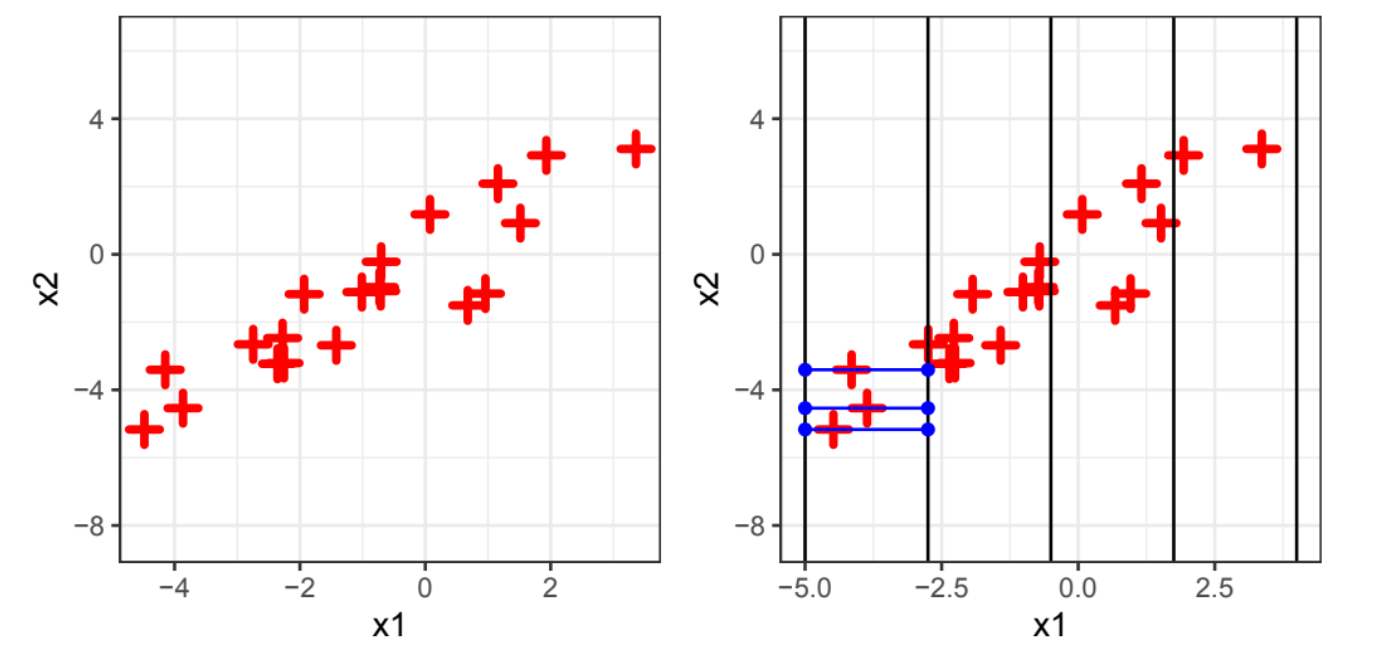
\includegraphics[width=0.5\textwidth]{figure/2D01.png}
\end{center}

\begin{itemize}
    \item avoids averaging predictions of unlikely data instances and blocks the effect of other correlated features.
    \pause
    \item divide the feature into intervals (vertical lines).
    \pause
    \item For the data instances in an interval, calculate the \textbf{difference in the prediction} when we replace the feature with the upper and lower limit of the interval (blue lines/points).
    \pause
    \item These differences are later accumulated and centered, resulting in the ALE curve.
\end{itemize} 

\end{frame}
%%%%%%%%%%%%%%%%%%%%%%%%%%%%%%%%%%%%%%%
\begin{frame}{2-D Illustration}
\vspace{-1em}
\begin{center}
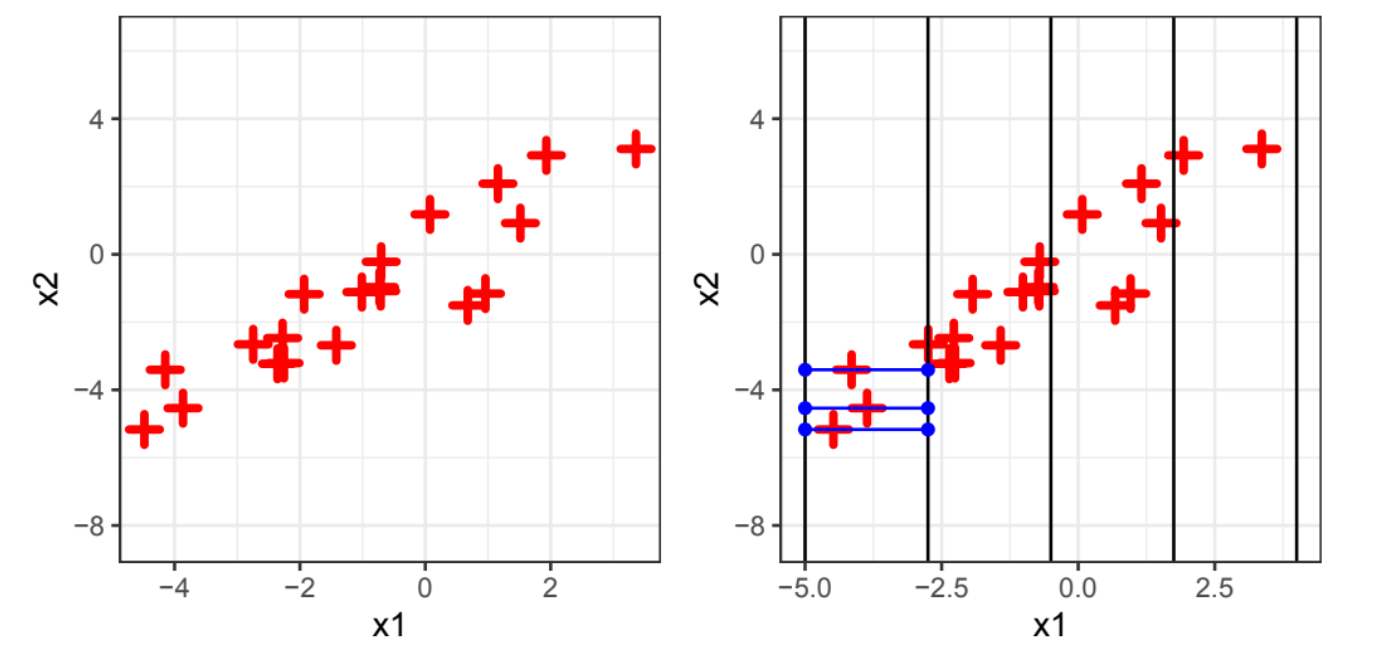
\includegraphics[width=0.5\textwidth]{figure/2D01.png}
\end{center}

\vspace{-1em}
Formally:
 \begin{itemize}
  \item  Consider the $i$-th observation $ x^{(i)} = (x_S^{(i)}, x^{(i)}_C)$. 
  \pause
  \item The observation's feature value $x_S^{(i)}$ is located within the $k$-th interval of $x_S$, i.e., $x_S^{(i)} \in \; ]z_{k-1, S}, z_{k, S}]$. 
  \pause
  \item We substitute $x_S^{(i)}$ by the right and left interval boundaries while $x^{(i)}_C$ is kept constant. 
  \pause
  \item The finite difference corresponds to $\hat{f}(z_{k, S}, x^{(i)}_C) - \hat{f}(z_{k-1, S}, x^{(i)}_C)$.
\end{itemize}


\end{frame}
%%%%%%%%%%%%%%%%%%%%%%%%%%%%%%%%%%%%%%%
\begin{frame}{2-D Illustration}
\vspace{-1em}
\begin{center}
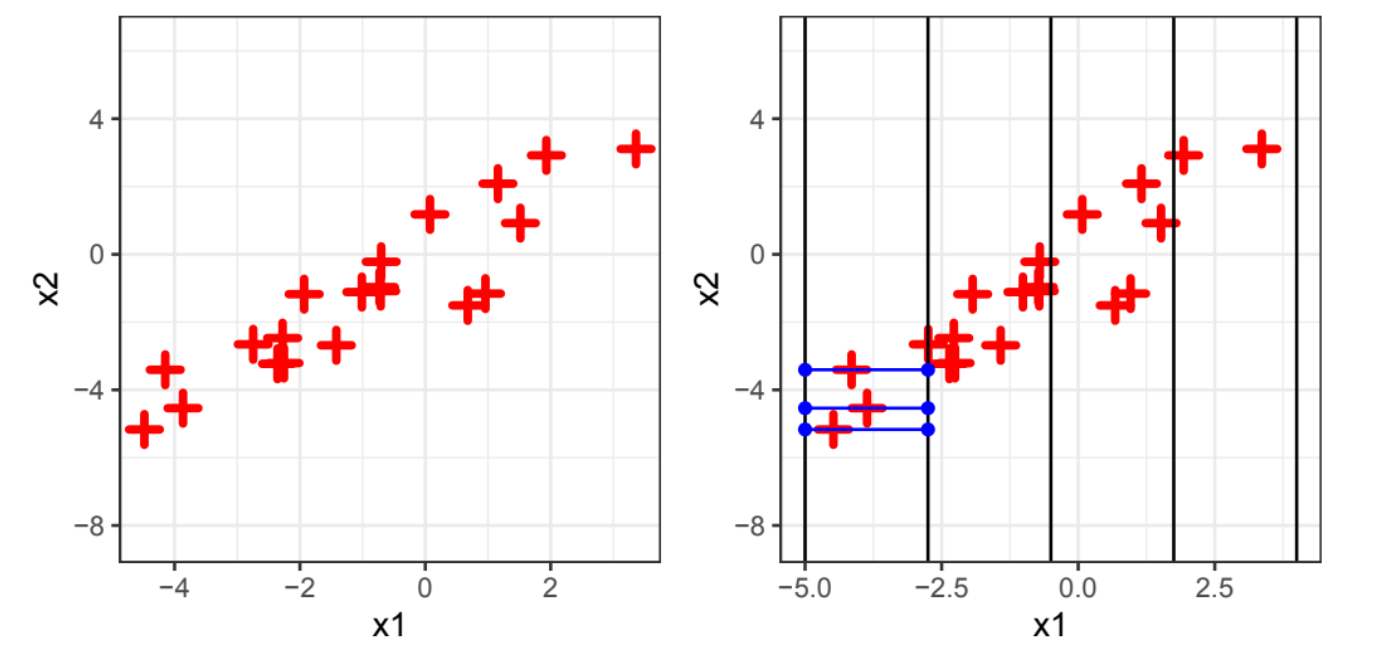
\includegraphics[width=0.5\textwidth]{figure/2D01.png}
\end{center}


 \begin{itemize}
  \item For each interval, we estimate the local effect by averaging all observation-wise finite differences. This replaces the inner integral, i.e., the integral with respect to the conditional distribution of $x_C$ on $x_S$.
  \item Summing up the local effects of all intervals up to the point of interest replaces the outer integral.
\end{itemize}

\end{frame}
%%%%%%%%%%%%%%%%%%%%%%%%%%%%%%%%%%%%%%%
\begin{frame}{ALE Estimation: Formula}

Let $k_S(x)$ denote the interval index a feature value $x \in x_S$ falls in. $n_S(k)$ denotes the number of observations inside the $k$-th interval of $x_S$. The estimated uncentered first order ALE $\hat{\tilde{f}}_{S, ALE}(x)$ at point $x$ corresponds to:
$$
\begin{aligned}
\hat{\tilde{f}}_{S, ALE}(x) = \sum_{k = 1}^{k_S(x)}\frac{1}{n_S(k)}\sum_{i: \; x_S^{(i)} \in \; ]z_{k-1, S}, z_{k, S}]}\left[\hat{f}(z_{k, S}, x^{(i)}_C) -\hat{f}(z_{k-1, S}, x^{(i)}_C)\right]
\end{aligned}
$$

\pause
In order to receive the centered ALE estimate $\hat{f}_{S, ALE}(x)$ at point $x$, we substract the average of the estimated uncentered ALE curve:

$$
\begin{aligned}
\hat{f}_{S, ALE}(x) = \hat{\tilde{f}}_{S, ALE}(x) - \frac{1}{n}\sum_{i = 1}^n \hat{\tilde{f}}_{S, ALE}(x_S^{(i)})
\end{aligned}
$$

\end{frame}
%%%%%%%%%%%%%%%%%%%%%%%%%%%%%%%%%%

\begin{frame}{ALE Estimation: Algorithm}

\begin{enumerate}
	\item \textbf{Sampling:} Create $K$ intervals for the value range of $x_S$.
	\item For each interval $k \in 1, \dots, k_S(x)$:
	  \begin{itemize}
	  \item Select the subset of observations inside the $k$-th interval.
	  \item \textbf{Intervention:} For each observation inside $k$-th interval: compute observation-wise finite difference.
	  \item \textbf{Prediction:} Average all observation-wise finite differences inside $k$-th interval to interval-wise local effect.
	  \end{itemize}
  \item \textbf{Aggregation:} Sum up all interval-wise local effects up to the point of interest $x$ for an uncentered ALE estimate.
  \item Center the uncentered ALE estimate.
\end{enumerate}

\end{frame}
%%%%%%%%%%%%%%%%%%%%%%%%%%%%%%%%%%%%%

\begin{frame}{Extrapolation and the ALE}
\begin{itemize}

\item Remember that there are two sources of extrapolation: 
\begin{enumerate}
    \item the model predicts in regions where it was not trained, and
    \item the Monte Carlo integral corresponds to an integration w.r.t. a uniform distribution, instead of the data distribution.
\end{enumerate} 
\pause\smallskip
\item Assuming that all interval boundaries are sufficiently close to the corresponding observed values, ALEs are robust to both sources of extrapolation.
  \begin{itemize}
    \item First, the trained model does not predict in regions where it was not trained.
    \item Second, we integrate with respect to the conditional distribution of $x_C$ on $x_S$ instead of the marginal distribution of $x_C$, by only averaging the finite differences inside a single interval.
  \end{itemize}
\end{itemize}
\end{frame}

	
\end{document}
